%\documentclass[10pt,twocolumn,letterpaper,draft]{article}
\documentclass[10pt,letterpaper]{article}

% 使用中文宏包
\usepackage[UTF8]{ctex}
\usepackage{graphicx} %插入图片的宏包
\usepackage{float} %设置图片浮动位置的宏包
\usepackage{subfigure} %插入多图时用子图显示的宏包
%\usepackage[utf8]{inputenc}
\usepackage[strings]{underscore}
\usepackage{times}
\usepackage{epsfig}
\usepackage{amsmath}
\usepackage{amssymb}
\usepackage{overpic}
\usepackage{listings}
\usepackage{color}
\usepackage{enumitem}
\setenumerate[1]{itemsep=0pt,partopsep=0pt,parsep=\parskip,topsep=5pt}
\setitemize[1]{itemsep=0pt,partopsep=0pt,parsep=\parskip,topsep=5pt}
\setdescription{itemsep=0pt,partopsep=0pt,parsep=\parskip,topsep=5pt}

\definecolor{mygreen}{rgb}{0,0.6,0}
\definecolor{mygray}{rgb}{0.5,0.5,0.5}
\definecolor{mymauve}{rgb}{0.58,0,0.82}
\lstset{ %
  backgroundcolor=\color{white},   % choose the background color
  basicstyle=\footnotesize,        % size of fonts used for the code
  breaklines=true,                 % automatic line breaking only at whitespace
  captionpos=b,                    % sets the caption-position to bottom
  commentstyle=\color{mygreen},    % comment style
  escapeinside={\%*}{*)},          % if you want to add LaTeX within your code
  keywordstyle=\color{blue},       % keyword style
  stringstyle=\color{mymauve},     % string literal style
}

% Include other packages here, before hyperref.

% If you comment hyperref and then uncomment it, you should delete
% egpaper.aux before re-running latex.  (Or just hit 'q' on the first latex
% run, let it finish, and you should be clear).
\usepackage[pagebackref=true,breaklinks=true,letterpaper=true,colorlinks,bookmarks=false]{hyperref}


\def\httilde{\mbox{\tt\raisebox{-.5ex}{\symbol{126}}}}

\newcommand{\cmm}[1]{\textcolor[rgb]{0,0.6,0}{CMM: #1}}
\newcommand{\todo}[1]{{\textcolor{red}{\bf [#1]}}}
\newcommand{\alert}[1]{\textcolor[rgb]{.6,0,0}{#1}}

\newcommand{\IT}{IT\cite{98pami/Itti}}
\newcommand{\MZ}{MZ\cite{03ACMMM/Ma_Contrast-based}}
\newcommand{\GB}{GB\cite{conf/nips/HarelKP06}}
\newcommand{\SR}{SR\cite{07cvpr/hou_SpectralResidual}}
\newcommand{\FT}{FT\cite{09cvpr/Achanta_FTSaliency}}
\newcommand{\CA}{CA\cite{10cvpr/goferman_context}}
\newcommand{\LC}{LC\cite{06acmmm/ZhaiS_spatiotemporal}}
\newcommand{\AC}{AC\cite{08cvs/achanta_salient}}
\newcommand{\HC}{HC-maps }
\newcommand{\RC}{RC-maps }
\newcommand{\Lab}{$L^*a^*b^*$}
\newcommand{\mypara}[1]{\paragraph{#1.}}

\graphicspath{{figures/}}

% Pages are numbered in submission mode, and unnumbered in camera-ready
%\ifcvprfinal\pagestyle{empty}\fi
\setcounter{page}{1}

\begin{document}
%\begin{CJK*}{GBK}{song}
 

%%%%%%%%% TITLE

\title{论文阅读笔记}

\author{纳文琪$^{1}$}

\maketitle

\section{概述}
\paragraph{} 卷积神经网络(Convotional Neural Network, CNN)是一种专门用于处理网格结构的神经网络,例如时间序列和图像。
CNN现在是图像处理领域
\section{CNN的发展历史}


\section{CNN}
\subsection{Network In Network\cite{networkinnetwor2013}}
\paragraph{} 传统的CNN采用卷积核与输入的数据块(data patch)进行内积,并将结果输入到激活函数来计算输出,这样的做法抽象能力不够。我们想要的结果是,相同概念的不同形式卷积后得出的抽象结果是不变的。论文通过在卷积核之后增加“微型网络”来提高抽象能力。
\begin{figure}[H] %H为当前位置,!htb为忽略美学标准,htbp为浮动图形
	\centering %图片居中
	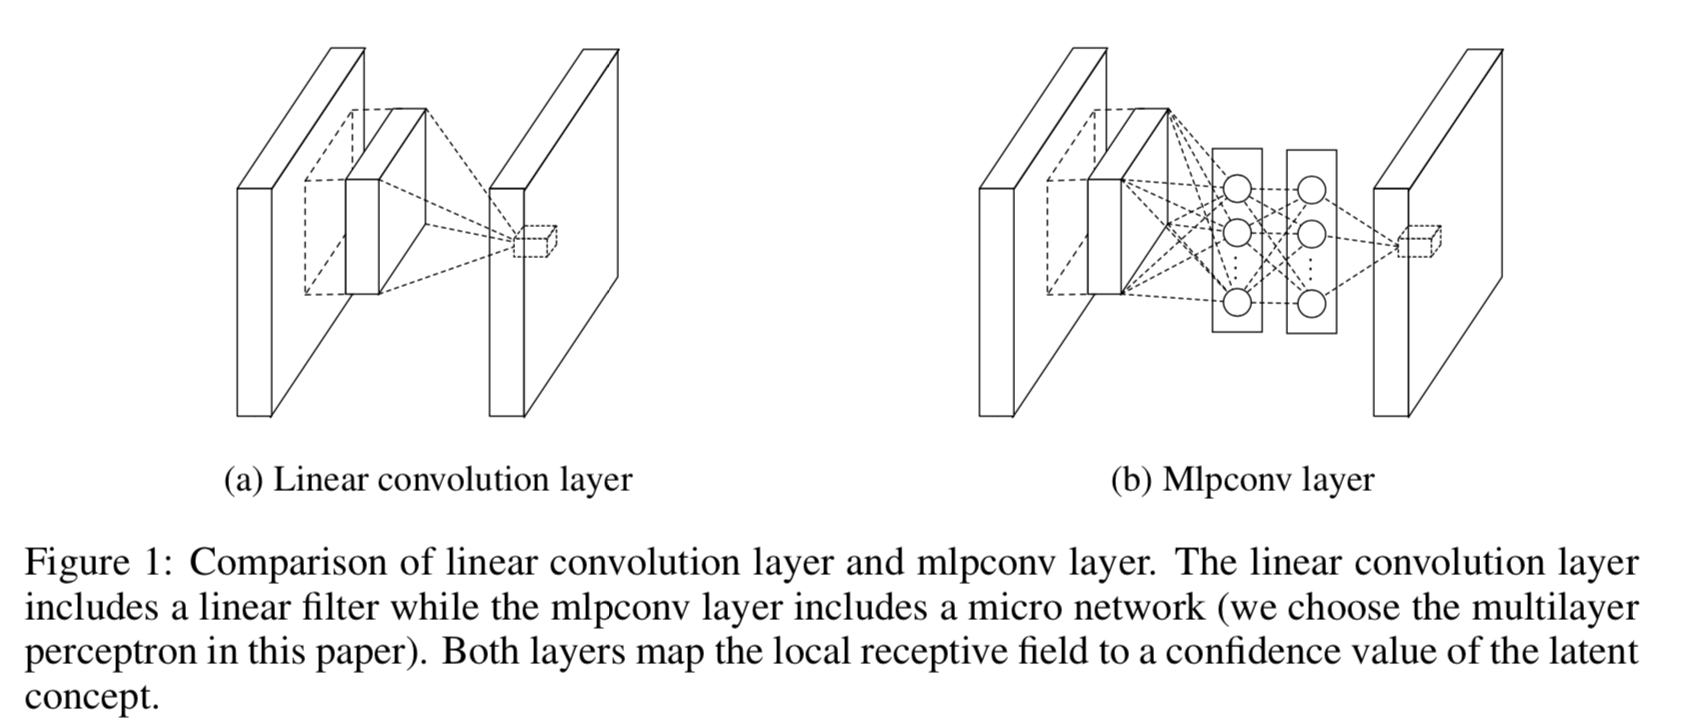
\includegraphics[width=0.7\textwidth]{images/nin-1.png} %插入图片,[]中设置图片大小,{}中是图片文件名
	\caption{} %最终文档中希望显示的图片标题
	\label{Fig.main2} %用于文内引用的标签
\end{figure}
也就是说,使用非线性模型来代替卷积的线性模型。
\paragraph{传统CNN} 传统的CNN网络使用卷积操作来计算特征图。计算通道$k$的特征映射中点$(i, j)$的值的公式是:
\begin{equation}
	f_{i,j,k} = \max(w_k^Tx_{i,j}, 0)
\end{equation}
首先将以$(i,j)$为中心的数据块与卷积核($w_k$)进行内积计算,再使用Relu进行激活。
\paragraph{MLP卷积层} 论文提到的mlpconv以另外的方式计算特征映射。
\begin{equation}
	f^1_{i,j,k_1} = \max ({w_{k_1}^1}^Tx_{i,j} + b_{k_1}, 0)
\end{equation}
\begin{equation}
	 f^n_{i,j,k_n} = \max ({w_{k_n}^n}^Tf_{i,j}^{n-1} + b_{k_n}, 0)
\end{equation}
$f_{i,j}^{n-1}$ 表示表示特征映射第n-1层所有通道的值的向量。也就是说,现在无论计算哪个通道上的特征映射的值都会与其他通道上的相同位置的点一同进行计算。这个跨通道池化(cross channel pooling)操作可简单地认为在卷积之后增加了一层$1 \times 1$的卷积,此时隐层的神经元数量与特征映射数量相等。
\paragraph{全局平均池化(Global Average Pooling)} 论文放弃了卷积层之后的全连接层,直接将最后一个特征图的空间平均(spatial average)作为分类置信度,再输入到最后的softmax中。这种做法可以替代dropout的使用。





















\bibliographystyle{ieeepes}
\bibliography{../Saliency}
\end{document}



























































